\documentclass[11pt,a4paper]{article}
\usepackage[margin=2.5cm]{geometry}
\usepackage[T1]{fontenc}
\usepackage{mathptmx}
\usepackage[utf8]{inputenc}

\usepackage{microtype}
\usepackage{booktabs}
\usepackage{tabularx}
\usepackage{graphicx}
\usepackage{amsmath}
\usepackage{xcolor}
\usepackage[numbers,sort&compress]{natbib}
\usepackage[hidelinks]{hyperref}
\usepackage{caption}
\captionsetup{font=small,labelfont=bf}
\setlength{\parskip}{0.4em}
\setlength{\parindent}{0pt}
\newcommand{\code}[1]{\texttt{#1}}

\title{\textbf{Serving-Aware Cost Modeling for Semantic Operators}\\[0.3em]
\large CMPE 491 Senior Project: Midterm Report}
\author{Yusuf Kaan Akçay\\
\small Advisor: Prof.\ Atay Özgövde\\
\small Department of Computer Engineering, Boğaziçi University}
\date{November 2026}

\begin{document}
\maketitle

\begin{abstract}
Semantic operator systems such as Palimpzest, with its optimizer Abacus, let users write queries
whose operators are executed by large language models (LLMs). The optimizer picks a physical plan
(which model runs which operator, and how) by estimating each operator's cost as tokens times API
price. When the same open models are served on one's own GPU with vLLM, the cost is GPU time
instead, and GPU time depends on batching, prefix-cache reuse and which model is resident in GPU
memory, none of which a token count sees. This project measures how far the two cost views
diverge. We built a portable harness that serves two 8B models on a single NVIDIA L4 GPU, switching
between them with vLLM's sleep mode, and ran four hand-fixed plans under two execution strategies on
the CUAD contract-review benchmark. Execution order alone changes GPU time by 7.8--11.5$\times$ at
identical token cost, and the plan that is cheapest at API prices (all-Llama) takes 58\% more GPU time
than the fastest plan (all-Qwen), which also has the highest F1. We also ran Abacus on the self-hosted models.
For the MaxQuality policy it again chose Mixture-of-Agents; executing that plan cost 9.9$\times$ more
at GPU prices than Abacus's API-price estimate, and the first run exposed serving problems
(unbounded outputs, a small KV cache) that we fix before the full Abacus run.
\end{abstract}

\section{Introduction}

LLM-powered query processing systems expose \emph{semantic operators}: map, filter, join or
extract steps whose logic is a natural-language instruction executed by an LLM. Palimpzest
\cite{palimpzest} and LOTUS \cite{lotus} are two such systems. Because a query can be executed in
many ways (different models per operator, ensembles such as Mixture-of-Agents, different prompt
strategies), these systems include a cost-based optimizer. Abacus \cite{russo2025abacus}, the
optimizer of Palimpzest, estimates the quality, cost and latency of candidate operators by sampling
them on a validation set and chooses a plan for a user policy such as ``maximize quality'' or
``minimize cost''.

The cost model is additive: an operator costs its input and output tokens times the model's API
price, and a plan costs the sum of its operators. This is accurate for a pay-per-token API. It is
not obviously accurate when an organization serves open models on its own GPUs, which is common for
privacy or volume reasons. There, the cost is GPU time, and GPU time for the same tokens depends on
(i)~how many requests the server can batch together, (ii)~how many prompt tokens are served from the
prefix cache, and (iii)~whether the model a step needs is already in GPU memory. Liu et
al.~\cite{liu2025optimizing} showed that reordering the rows and columns of an LLM query increases
prefix-cache reuse and speeds it up by up to 3.4$\times$ without changing the token count, an effect
a token-based estimate cannot see.

This report presents the research question and hypotheses (Section~\ref{sec:rq}), related work
(Section~\ref{sec:related}), the experimental method (Section~\ref{sec:method}), the measurement
infrastructure (Section~\ref{sec:impl}), results so far (Section~\ref{sec:results}), and the plan for
the rest of the project (Section~\ref{sec:plan}).

\section{Research Question and Hypotheses}\label{sec:rq}

\textbf{Research question.} Does a semantic query plan that is optimal under API pricing remain
optimal when executed on a self-hosted vLLM server, and if not, how far do the two cost views
diverge?

\begin{table}[h]
\centering\small
\begin{tabularx}{\linewidth}{@{}lXX@{}}
\toprule
& Hypothesis & Test \\
\midrule
H1 & The self-hosted cost of multi-model plans (mixed, Mixture-of-Agents) depends on execution order; switching models per record can push them off the Pareto frontier. & Run the same plan record by record and operator by operator; compare GPU time and model switches. \\
H2 & Running operators that share a model back to back increases prefix-cache reuse, which an additive cost model ignores. & Measure prefix-cache hits and GPU time with the token count fixed. \\
H3 & Plans ranked by API cost and by GPU cost are ordered differently. & Kendall's $\tau$ between the two rankings; compare the two Pareto frontiers. \\
\bottomrule
\end{tabularx}
\caption{Hypotheses.}
\end{table}

\section{Related Work}\label{sec:related}

We followed the citation trees of the two papers above three levels deep on Semantic Scholar (56
direct citations, about 2,170 papers in total), filtered them by keyword, and read the closest
$\sim$20 papers. The search and screening were done with the help of an AI assistant (Claude).

Two lines of work exist side by side (Table~\ref{tab:related}). Systems that \emph{choose} a plan do
not model the serving state of the GPU (which model is loaded, what is cached); systems that
\emph{execute} LLM workloads efficiently on GPUs take the plan as given. We found no work that
measures this gap for semantic operator optimizers. The contribution of this project is therefore a
measurement, not a new system.

\begin{table}[h]
\centering\small
\begin{tabularx}{\linewidth}{@{}llX@{}}
\toprule
Work & Side & Relation to this project \\
\midrule
Halo \cite{halo} & Execution & Cost model covers prefill/decode, cache sharing and model loading, but takes the model assignment as given. \\
Kalypso \cite{kalypso} & Execution & Shares KV cache across semantic operators; single model, no plan choice. \\
Helium \cite{helium} & Execution & Cache- and batch-aware scheduling; single model. \\
MOSAIC \cite{mosaic} & Execution & Schedules Mixture-of-Agents on limited GPUs; no plan choice. \\
Stretto \cite{stretto} & Plan choice & Models operator cost by measured time; no model switching, no API vs.\ GPU comparison. \\
BlendSQL v0.1.0 \cite{blendsql} & Plan choice & Compares open models on a local GPU with APIs; rule-based optimizer. \\
AI$\times$DB / NeurEngine \cite{aixdb} & Vision & Names model placement outside the optimizer as an open problem. \\
Akillioglu \cite{akillioglu2025} & Vision & Proposes a cost model that includes KV-cache hits; SQL, single model. \\
Multi-model schedulers \cite{multimodelsched} & Switching & Reports 4--5\,s to reload an 8B model. \\
\bottomrule
\end{tabularx}
\caption{Closest related work.}\label{tab:related}
\end{table}

\section{Method}\label{sec:method}

\subsection{Two experiments}

\textbf{Control experiment (hand-fixed plans).} We fix four plans and two execution strategies
ourselves. Because we choose the plans, we can isolate the effect of batching, prefix caching and
model switching. Its results also serve as the reference for interpreting the plans Abacus chooses.

\textbf{Main experiment (Abacus).} We give Abacus the API list prices of the two models and let it
choose a plan for each policy (MaxQuality, MinCost, MinTime). We then execute the chosen plan on the
self-hosted server and measure its GPU time.

In both, every plan is priced twice: tokens $\times$ API list price, and measured GPU time $\times$
hourly GPU price. The two rankings are compared with Kendall's $\tau$ and two Pareto frontiers
(quality against each cost).

\subsection{Models, plans and strategies}

The models are Llama-3.1-8B-Instruct and Qwen2.5-7B-Instruct. API prices are Together AI list
prices: 0.18\,USD per million tokens for Llama-3.1-8B and 0.30\,USD for Qwen2.5-7B-Turbo, for both
input and output \cite{togetherllama,togetherqwen}. The GPU price is the on-demand price of the
\code{g2-standard-16} VM (one L4, 16 vCPUs, 64\,GB RAM), 1.147\,USD per hour
\cite{gcppricing}; this is the price of the whole VM, not only the GPU.

\begin{table}[h]
\centering\small
\begin{tabularx}{\linewidth}{@{}lX@{}}
\toprule
Plan & Definition \\
\midrule
\code{all\_llama} & Both operators run on Llama. \\
\code{all\_qwen} & Both operators run on Qwen. \\
\code{mixed} & One model per operator (operator A on Qwen, operator B on Llama). \\
\code{moa} & Operator A on Qwen; operator B as Mixture-of-Agents: Llama and Qwen propose, Llama aggregates. \\
\midrule
Strategy & Definition \\
\midrule
\code{naive} & Record by record; switches the model whenever the next step needs the other one. \\
\code{batched} & Operator by operator; each model is woken once and processes all records. \\
\bottomrule
\end{tabularx}
\caption{Plans and execution strategies of the control experiment.}
\end{table}

Single-model plans never switch models, so their naive/batched gap isolates batching and caching;
for multi-model plans the switch cost comes on top.

\subsection{Workload: CUAD}

CUAD \cite{hendrycks2021cuad} is a legal contract-review dataset with 41 clause categories (for
example parties, governing law, non-compete) annotated as text spans. We select 25 test contracts
exactly as Abacus's CUAD demo does (titles shuffled with seed 0) and split them into chunks of at most
4,000 characters, giving 160 chunks; 99\% of the labeled spans fall inside a single chunk. For
Abacus's sampling we prepare 25 training contracts the same way (313 chunks). In the control
experiment the 41 categories are extracted by two operators (21 and 20 categories); in the Abacus
experiment by Abacus's own single operator over all 41.

Quality is precision, recall and F1 with Abacus's span matching (a prediction matches a label when
their Jaccard similarity is at least 0.15; for Parties a substring also counts), with predictions
merged per contract. Our implementation agreed with Abacus's \code{evaluate\_entry} on 3,000 random
cases.

\subsection{What is held fixed and what is measured}

Held fixed: the config (its hash is stored with every run), GPU type, vLLM version (0.30.0), image
digest, temperature 0, and an empty prefix cache with the first model awake at the start of every
run. Measured: wall-clock GPU time, number and duration of model switches, prompt, completion and
cached tokens per model, prefix-cache queries and hits from vLLM's \code{/metrics}, and F1.

\section{Measurement Infrastructure}\label{sec:impl}

\textbf{Harness.} One Docker image (the official vLLM image plus our harness), one YAML config and
one command. The runner starts one vLLM server per model and keeps exactly one awake using vLLM's
sleep mode \cite{kwon2023vllm}: a sleeping server moves its weights to CPU memory and drops its KV
cache, so two 8B models share one 24\,GB L4. Every (plan, strategy, repeat) combination is run from
the same starting state and appended as one JSON line. Runs have deterministic IDs, so an interrupted
experiment resumes where it stopped. The same image runs on a laptop, a GCP VM, TRUBA (Slurm and
Apptainer) or Kubernetes; only the launcher differs.

\textbf{GCP pipeline.} A launcher uploads the config to Cloud Storage and starts a Cloud Build job
that builds the image and creates the GPU VM, retrying zones in six regions because L4 GPUs are
frequently out of stock. The VM's startup script pulls the image, restores earlier results, runs the
harness, uploads results with memory and kernel logs, and deletes itself. VMs have no external IP.
Spending is capped: a budget on cost after credits triggers a Cloud Run function that disables
billing for the project.

\textbf{Measurement checks.} On a laptop GPU (RTX 3050 Ti, 4\,GB) and later on the L4 we verified that
vLLM exposes every quantity we need: per-request cached prompt tokens, server-wide prefix-cache
counters, a prefix-cache reset endpoint, and sleep/wake endpoints. The per-request cached-token
counts and the server counters agreed in every run.

\textbf{Abacus integration.} Palimpzest 1.5.3 runs in its own Python environment inside the image and
sends requests for both models to a small proxy we wrote, which exposes one OpenAI-compatible
endpoint, wakes the requested model and batches concurrent requests for the awake model. Running
Abacus on self-hosted models needed six changes, all applied at runtime without modifying the
installed package:
\begin{enumerate}\itemsep0em
\item Palimpzest allows only one vLLM model per query; this check is lifted.
\item vLLM models are priced at zero; they receive the API list prices from our config.
\item Palimpzest records zero input tokens for vLLM models, so cost estimates counted only output
tokens. We count every prompt token at the input price, as an API without a cache discount would.
\item The default validator calls an OpenAI model; ours scores sampled outputs against the CUAD
labels of the training chunks.
\item Palimpzest sets no output-token limit. The proxy adds one (2,048 tokens) to requests without
a limit (introduced after the first run; Section~\ref{sec:abacusres}).
\item Model priors (MMLU-Pro score, speed) are predicted from the Hugging Face model ID rather than
the short served name, which had given both models the same prior.
\end{enumerate}
The integration was tested end to end against a stub vLLM server (Section~\ref{sec:abacusres}).

\section{Results}\label{sec:results}

All runs use one NVIDIA L4 on a \code{g2-standard-16} VM and vLLM 0.30.0. Each result is read from
the run's \code{runs.jsonl} in the project bucket.

\subsection{First measurements (small workload)}

A small test workload (six reviews, two operators, 3 repeats differing by less than 1\%) with the two
8B models showed the effects in their purest form (Table~\ref{tab:smoke}). One model switch takes
3.03\,s, and under the naive strategy switches account for 89--91\% of the run time of the
multi-model plans. Switching also discards the prefix cache: \code{mixed} under naive gets no cached
prompt tokens, against 320 under batched.

\begin{table}[h]
\centering\small
\begin{tabular}{@{}lrrrr@{}}
\toprule
Plan & naive (s) & batched (s) & Ratio & Switch time, naive \\
\midrule
\code{all\_llama} & 4.92 & 0.99 & 5.0$\times$ & -- \\
\code{all\_qwen}  & 4.28 & 0.91 & 4.7$\times$ & -- \\
\code{mixed}      & 37.27 & 3.91 & 9.5$\times$ & 33.3\,s (89\%) \\
\code{moa}        & 39.76 & 6.85 & 5.8$\times$ & 36.4\,s (91\%) \\
\bottomrule
\end{tabular}
\caption{Small test workload with Llama-3.1-8B and Qwen2.5-7B (mean of 3 repeats).}\label{tab:smoke}
\end{table}

These runs also exposed two constraints of serving two 8B models on one L4. First, vLLM's memory
budget (\code{gpu\_memory\_utilization}) must leave room for the sleeping server, which still holds about
1.8\,GiB of GPU memory (0.80 left no KV cache for Llama, 0.90 did not fit, 0.85 works). Second, the runs
failed on VMs with 32\,GB and 48\,GB of host RAM and succeeded with 64\,GB.

\subsection{CUAD control experiment}

A pilot on the first 40 chunks (6 contracts) confirmed the setup and measured throughput; the full
run on all 160 chunks took 7.7 hours of GPU time for the eight runs (one repeat).
Table~\ref{tab:cuad} gives the full run.

\begin{table}[h]
\centering\small
\begin{tabular}{@{}llrrrrrr@{}}
\toprule
Plan & Strategy & GPU time (s) & Switches (n / s) & Cache hit & F1 & API (USD) & GPU (USD) \\
\midrule
\code{all\_qwen}  & batched & 352.5   & 0 / 0         & 54\% & 0.665 & 0.155 & 0.112 \\
\code{mixed}      & batched & 447.6   & 1 / 3.1       & 54\% & 0.656 & 0.123 & 0.143 \\
\code{all\_llama} & batched & 557.5   & 0 / 0         & 55\% & 0.645 & 0.093 & 0.178 \\
\code{moa}        & batched & 1,255.8 & 3 / 9.2       & 47\% & 0.550 & 0.248 & 0.400 \\
\midrule
\code{all\_qwen}  & naive   & 4,055.5 & 0 / 0         & 54\% & 0.663 & 0.155 & 1.292 \\
\code{all\_llama} & naive   & 4,374.1 & 0 / 0         & 55\% & 0.653 & 0.093 & 1.394 \\
\code{mixed}      & naive   & 5,129.7 & 319 / 973.6   & 0\%  & 0.654 & 0.123 & 1.635 \\
\code{moa}        & naive   & 11,526.2 & 639 / 1,949.6 & 0\% & 0.555 & 0.248 & 3.673 \\
\bottomrule
\end{tabular}
\caption{CUAD, 25 contracts (160 chunks), one repeat. Cache hit is cached prompt tokens over prompt
tokens. API cost is prompt and completion tokens times the list prices; GPU cost is GPU time times
the hourly VM price.}\label{tab:cuad}
\end{table}

\begin{figure}[h]
\centering
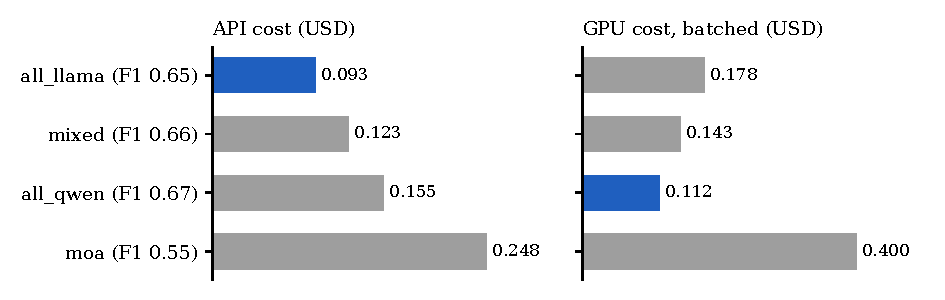
\includegraphics[width=\linewidth]{fig/ranking.pdf}
\caption{The same four plans (batched) ordered by API cost. The cheapest plan in each view is
highlighted: all-Llama at API prices, all-Qwen on the GPU.}\label{fig:ranking}
\end{figure}

\begin{figure}[h]
\centering
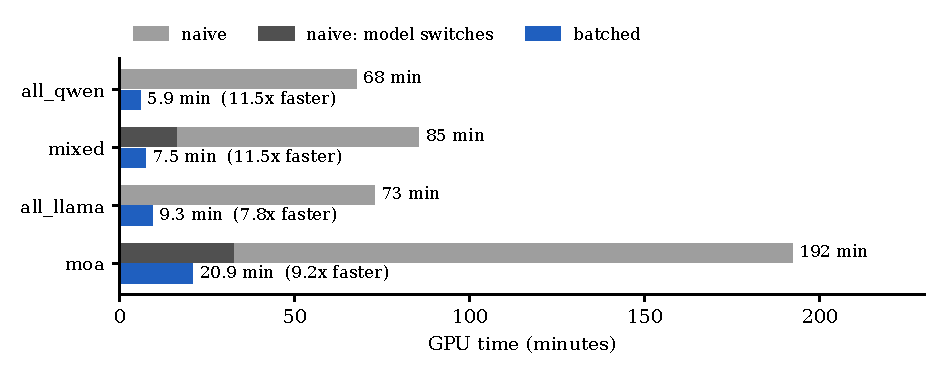
\includegraphics[width=\linewidth]{fig/strategies.pdf}
\caption{GPU time of each plan under the two strategies. Both strategies use the same tokens, so the
API cost of a plan is the same for both.}\label{fig:strategies}
\end{figure}

\textbf{Finding 1: the cheapest plan at API prices is not the cheapest on the GPU (H3).} At API
prices the order is all-Llama, mixed, all-Qwen, MoA; on the GPU (batched) it is all-Qwen, mixed,
all-Llama, MoA (Figure~\ref{fig:ranking}). All-Llama costs 60\% of all-Qwen at API prices but takes
58\% more GPU time, while both plans use almost the same tokens (443k and 445k prompt tokens). The
difference therefore comes from how fast each model is served, not from the token count. A possible
cause, not yet measured, is the KV-cache footprint: 128\,KiB per token for Llama-3.1-8B against
56\,KiB for Qwen2.5-7B, so the same memory holds more concurrent Qwen requests. Kendall's $\tau$
between API cost and GPU time is 0.0 for the batched plans and 0.33 for the naive ones, with only four
plans per ranking.

\textbf{Finding 2: execution order changes GPU time by an order of magnitude at identical API cost
(H1).} Every plan uses the same tokens under both strategies, yet naive takes 7.8--11.5$\times$
longer than batched (Figure~\ref{fig:strategies}). An API cost model assigns both the same cost.

\textbf{Finding 3: at CUAD scale, switching is secondary to batching and caching (H1, H2).} Model
switches take 17--19\% of the naive run time of the multi-model plans, down from 89--91\% on the small
workload, because each record now carries far more work. The larger loss is that naive execution
processes records one at a time, and that every switch empties the prefix cache: naive \code{mixed}
and \code{moa} get no cache hits, against 47--54\% under batched.

\textbf{Finding 4: Pareto frontiers.} With F1 against API cost, all-Llama, mixed and all-Qwen are on
the frontier. With F1 against GPU cost (batched), all-Qwen dominates every other plan, so the
frontier is a single point. MoA, which Abacus selected in all ten of its CUAD trials with API models
\cite{russo2025abacus}, is dominated in both views here: it uses twice the tokens, has the lowest F1
(0.55) and the longest GPU time.

\subsection{Abacus on the self-hosted models}\label{sec:abacusres}

The integration was first tested end to end against a stub vLLM server. The first run on the L4
(all 160 test chunks, sample budget 50, policies MaxQuality, MinCost and MinTime) completed only the
MaxQuality policy before the VM reached its 6-hour limit (Table~\ref{tab:abacus}).

\begin{table}[h]
\centering\small
\begin{tabular}{@{}lrrrrr@{}}
\toprule
Phase & GPU time (s) & Switches (n / s) & API (USD) & GPU (USD) & GPU / API \\
\midrule
Optimization (train chunks) & 4,315.7 & 50 / 151.4 & 0.189 & 1.375 & 7.3$\times$ \\
Execution (160 test chunks)              & 7,303.8 & 10 / 32.9  & 0.235 & 2.328 & 9.9$\times$ \\
\bottomrule
\end{tabular}
\caption{Abacus, MaxQuality policy. Chosen plan: one Mixture-of-Agents operator over all 41
categories, proposers Llama and Qwen, aggregator Qwen. API cost is Palimpzest's own figure at the list
prices; GPU cost is GPU time times the hourly VM price. Source: \code{results/cuad-25-pz/pz\_runs.jsonl}.}
\label{tab:abacus}
\end{table}

\textbf{Abacus again chooses Mixture-of-Agents.} As in all ten of its CUAD trials with API models
\cite{russo2025abacus}, MaxQuality selected a Mixture-of-Agents operator, the plan type that is
dominated in our control experiment.

\textbf{The API estimate misses the GPU cost by an order of magnitude.} Executing the plan cost
2.33\,USD at GPU prices against 0.24\,USD at API prices (9.9$\times$); for the hand-fixed
Mixture-of-Agents plan in the control experiment the ratio was 1.6$\times$ (batched).

\textbf{The serving logs explain why.} vLLM could allocate only 9,040 tokens of KV cache to Llama
(32,992 to Qwen), so Llama served about one long request at a time, at about 16 output tokens per
second. Palimpzest sets no output limit, and when the run stopped a single running Llama request occupied about 90\% of that cache. The
client timed out on 358 requests after 600\,s, and 34 answers could not be parsed. These failures
likely lower quality as well: F1 was 0.31 (precision 0.59, recall 0.21), so this F1 is not comparable with the
control experiment. The proxy now adds an output limit, and a pilot on 20 chunks will measure the run
time before the full Abacus run is repeated.

\section{Limitations}

\begin{itemize}\itemsep0em
\item The CUAD runs have a single repeat. On the small workload repeats differed by less than 1\%;
additional repeats of the batched runs are planned.
\item Each ranking has four plans, so Kendall's $\tau$ is a weak statistic here; the per-plan
comparison is the main evidence.
\item The GPU price is the price of the whole VM. A different GPU or price would change the absolute
GPU costs but not the ranking by GPU time.
\item Both models share one GPU in every run, including single-model plans, so the sleeping model
reduces the KV cache available to the active one. Running single-model plans with one server may be
the fairer baseline.
\item The cause of the host-RAM failures on smaller VMs has not been identified.
\item The first Abacus run covers one policy and suffered from timeouts; its cost ratio reflects
our serving setup as much as the plan, and its F1 is not reliable.
\end{itemize}

\section{Plan for the Rest of the Project}\label{sec:plan}

\begin{enumerate}\itemsep0em
\item Run the Abacus pilot with the output limit, then the full run with all three policies, and
compare the plan Abacus chooses for each policy with its GPU cost and with the control experiment.
\item Increase the KV cache available to Llama next to the sleeping model (for example an FP8 KV
cache), and measure its effect on the control experiment as well.
\item Repeat the batched CUAD runs to report variance.
\item Test the KV-cache explanation of Finding~1 (concurrency and KV-cache size per model).
\item Run single-model plans with one server loaded, as an alternative baseline.
\item Profile host and GPU memory around model switches.
\item If time permits, add a second workload to test whether the findings generalize beyond CUAD.
\end{enumerate}

The code is available at \url{https://github.com/akcayyusufkaan/serving-aware-semantic-ops}.

\bibliographystyle{plainnat}
\bibliography{refs}

\end{document}
